\documentclass[12pt,a4paper]{article}
\usepackage[14pt]{extsizes}
\usepackage[french]{babel}
\usepackage[utf8]{inputenc}
\usepackage[T1]{fontenc}
\usepackage{wrapfig}
\usepackage{array}
\usepackage{graphicx}

\title{}
\author{}
\date{}

\newcommand{\subtitle}{Rapport de soutenance II}

\begin{document}
	\begin{titlepage}
	\begin{center}
	\vspace{8cm}
	
\includegraphics[width=15cm]{images/spacesymphonia.png}

	\vspace{0.5cm}
	\LARGE{\textbf{\subtitle}}

	\vspace{1cm}
	\large{\textsf{
	Emmanuel `Green` \bsc{Guet} \\
	Antoine `Nervous` \bsc{Vallée} \\
	Antoine `serialk` \bsc{Pietri}}}

	\vspace{2cm}

	\large{\textsf{Projet d'InfoSup --- EPITA}}

	\end{center}
	\end{titlepage}

	\setcounter{tocdepth}{3}
	\tableofcontents
	\newpage
	\pagestyle{headings}

	\section{Introduction}
		\par
		Ce rapport contient la quasi-intégralité du travail effectué par l'équipe \texttt{TEUH TEUH TEUH} sur le projet de jeu \emph{Space Symphonia} pendant les 7 semaines d'intervalle entre les deux premières soutenances. \\
		\par
		Comme pendant la première soutenance, l'essentiel de notre travail s'est concentré sur ce qui avait été annoncé dans le premier cahier des charges, c'est à dire les points suivants : \\
		\par
		\begin{itemize}
		\item Ajout de contenu (ennemis, missiles, boss) ;
		\item Mode Extrême
		\item Amélioration et complétion de l'interface et du menu
		\item Début d'implémentation d'obstacles
		\item Amélioration des graphismes et particules, et de l'esthétique du jeu
		\item Analyse sonore entraînant des modifications des mécanismes du jeu
		\item Création du site Web.
		\end{itemize}
		\newpage
	\section{Nouveaux mécanismes et nouveau contenu}
		\subsection{Nouveaux ennemis}
		Voici la liste des nouveaux ennemis ajoutés jusqu'ici :
		\begin{itemize}
			\item[$\bullet$ Drone]
				\par~
				\begin{itemize}
					\item Vie : 20
					\item Dommages en cas de collision : 30
					\item Vitesse : Rapide
					\item Tir : Blaster
					\item Dangerosité : 5%
				\end{itemize}
				\par~
			\item[$\bullet$ Double Shooter]
				\par~
				\begin{itemize}
					\item Vie : 40
					\item Dommages en cas de collision : 30
					\item Vitesse : Rapide
					\item Tir : Blaster ($\times2$)
					\item Dangerosité : 10%
				\end{itemize}
			\item[$\bullet$ Energizer]
				\par~
				\begin{itemize}
					\item Vie : 50
					\item Dommages en cas de collision : 30
					\item Vitesse : Moyenne
					\item Tir : Boule d'énergie
					\item Dangerosité : 15%
				\end{itemize}
				\par~
			\item[$\bullet$ Kamikaze]
				\par~
				\begin{itemize}			
					\item Vie : 5
					\item Dommages en cas de collision : 100
					\item Vitesse : Très rapide
					\item Tir : Aucun
					\item Dangerosité : 25%
				\end{itemize}
				\par~
		\end{itemize}
		
		\newpage
		\subsection{Nouveaux missiles}
		Voici la liste des nouveaux missiles ajoutés jusqu'ici :
		\begin{itemize}
			\item[$\bullet$ Blaster]
				\par~
				\begin{itemize}
					\item Dégats : 20
					\item Vitesse : Rapide
				\end{itemize}
				\par~
			\item[$\bullet$ Boule d'énergie]
				\par~
				\begin{itemize}
					\item Dégats : 50
					\item Vitesse : Moyenne
				\end{itemize}
		\end{itemize}
		\subsection{Obstacles}		
		\par 
		Nous avons commencé à implémenter des obstacles dans le jeu. Jusqu'ici nous n'avons ajouté qu'un trou noir, qui attire tous les vaisseaux en son centre, mais il n'est pas encore fonctionnel dans le jeu.
		\subsection{Menu}
		\par
		Le menu est désormais complètement fonctionnel, même si nous y rajouterons des options au fur et à mesure des besoins.
		\begin{center}
		\vspace{0.5cm}
		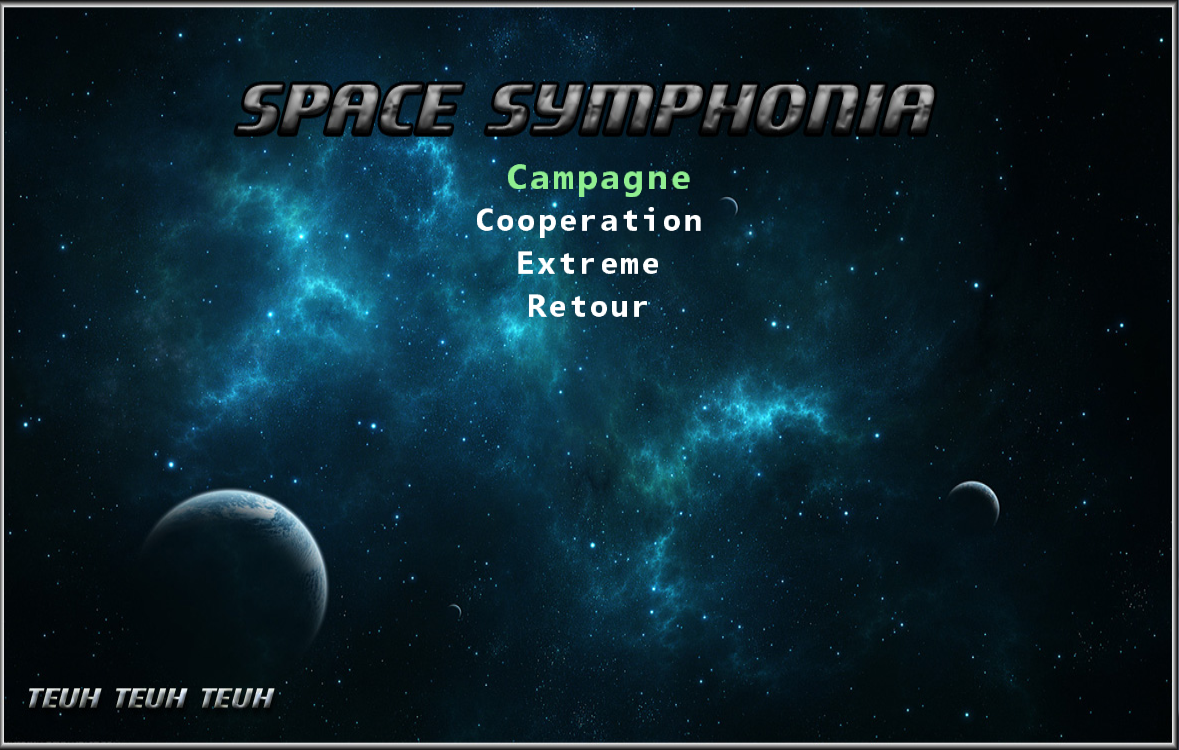
\includegraphics[width=350pt]{images/menu1.png}
		\end{center}
		\newpage
		\subsubsection{Scores}
		\par
		Le joueur a désormais la possibilité de consulter ses scores via un tableau disponible dans le menu.
		Il lui suffit de choisir son mode de jeu, puis le meilleur score de chaque niveau est affiché.
		Ensuite, il ne lui reste plus qu'à choisir un niveau pour accéder à plus de détails, et il peut ainsi consulter les 5 meilleures scores de chaque niveau, et le pseudonyme de celui qui les a obtenus.
		\begin{center}
		\vspace{1cm}
		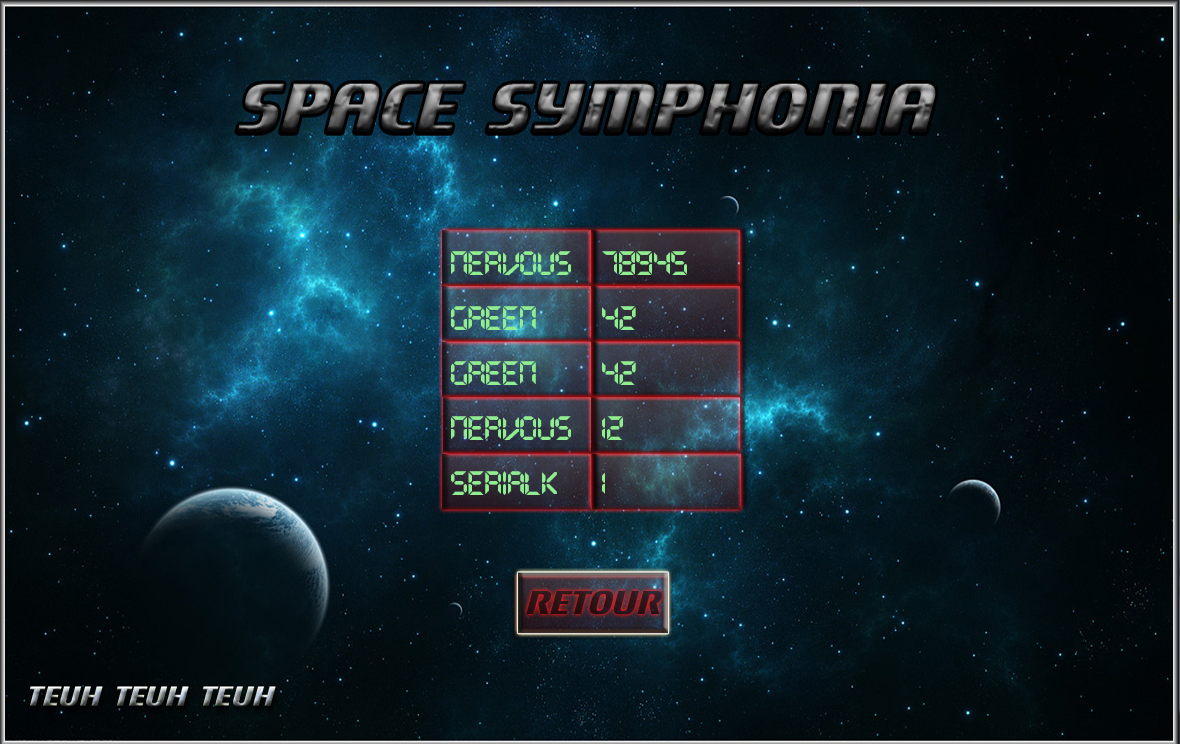
\includegraphics[width=400pt]{images/score1.png}
		\vspace{1cm}
		\end{center}
		
		\subsubsection{Sélection de niveau}
		\par
		Nous avons ajouté un menu de sélection de mode de jeu, puis de niveaux. Les niveaux sont divisés en plusieurs actes, divisés eux-mêmes en plusieurs niveaux.
		Notre menu vous propose de choisir votre mode de jeu, puis le niveau à jouer.
		Le niveau est ensuite chargé automatiquement, et prend fin une fois réussi (ou \emph{perdu}), ou lorsque vous le quittez dans le menu de pause (touche \texttt{ECHAP}).
		
		\subsection{Boss}
		\par
		Nous avons ajouté au jeu un tout nouveau type d'ennemis : les Boss.
		Ils viendront « pimenter » votre partie, et rendre le jeu plus dynamique.
		Ils apparaissent en milieu ou en fin de partie, mais attendez vous à en croiser régulièrement.
		\par
		Les Boss ont évidemment un nombre bien plus important de points de vie que les ennemis normaux, une texture unique pour chacun d'eux, et ils vous feront mordre la poussière à plusieurs reprises si vous ne comprenez pas la tactique qui vous permettra de les vaincre.
		
		\subsubsection{Intelligence artificielle}
		\par
		Les Boss nous ont amené à inclure dans le jeu un début d'IA, pour régir leurs mouvements et leurs attaques.
		Ils n'ont en effet pas les même compétences en fonction de la durée du combat ou de leurs points de vie:
		Il est possible, si vous ne les tuez pas assez vite, qu'ils vous envoient un missile qui peut vous tuer en un coup.
		\par
		Nous avons voulu rendre nos ennemis plus vivants, et ainsi chaque boss possède différentes phases. 
		Ces phases sont déterminées en fonction de la vie du boss, du temps écoulé\ldots~ Elles indiquent au Boss quels déplacements et quels missiles utiliser à tout instant.
		\begin{center}
			\vspace{1cm}
			
			\includegraphics[width=400pt]{images/phase1.png}
			\par \emph{Un exemple de la phase 1 du premier boss}
			
			\vspace{0.4cm}
	
			\includegraphics[width=400pt]{images/phase2.png}
			\par \emph{Phase 2 du premier boss: changement de tactique}
	
			\vspace{0.4cm}
			
			\includegraphics[width=400pt]{images/phase22.png}
			\par \emph{Changement d'arme du premier boss}
			
			\vspace{0.4cm}
		\end{center}
		
		\subsection{Interface}
		\par
		Une interface est désormais implémentée dans le jeu.
		Cette dernière permet pour l'instant de connaitre la vie du joueur, son score, mais aussi d'obtenir des informations sur le boss contre lequel le joueur est en train de se battre.
		\par
		Nous avons souhaité limiter au maximum le nombre d'informations à l'écran, afin de ne pas nuire à la visibilité du jeu, et à prolonger son immersion.
		C'est pourquoi toutes les informations vitales au joueur sont concentrées en bas de l'écran, dans une interface peu encombrante et bien pensée.
		\begin{center}
		\vspace{1cm}
		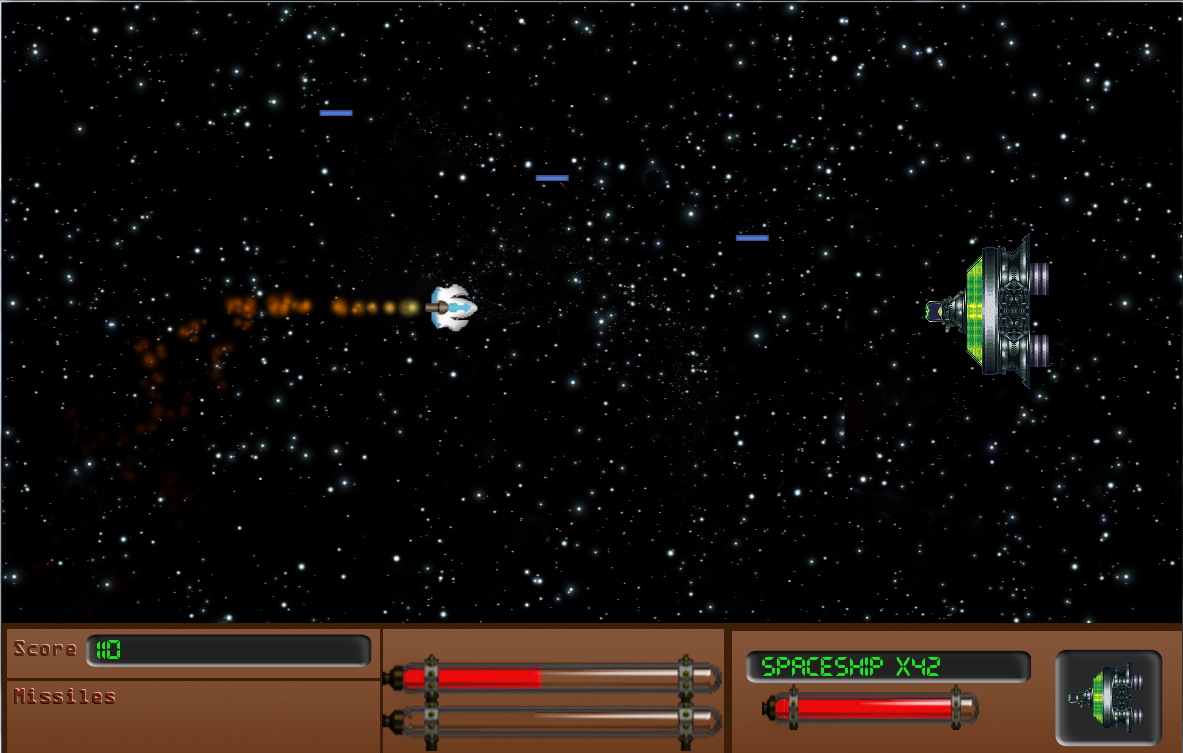
\includegraphics[width=400pt]{images/hud1.png}
		\vspace{1cm}
		\end{center}
		
		\newpage
		\subsection{Mode extrême}
		Le mode extrême a été implémenté mais n'a pour l'instant pas d'intérêt puisqu'il ne permet que de tuer le seul boss disponible à ce jour.
		Il sera amélioré dans le futur, par l'ajout des nouveaux boss qui feront leur apparition dans le jeu.
	
		\subsection{Analyse sonore}
		\subsubsection{Théorie : Récupération de l'énergie musicale}
		Nous avons également progressé dans notre analyse sonore. Pendant la soutenance précédente nous avions réalisé un spectre qui traduisait à chaque instant les amplitudes moyennes de la musique. Or, après plusieurs recherches, nous avons trouvé comment extraire, à partir de ces amplitudes, l'\emph{énergie} de la musique à un instant précis.
		FMOD nous permet d'obtenir un tableau de $2^k$ amplitudes correspondant chacune à une fréquence de chaque sortie audio toutes les 25 millièmes de secondes. Pour obtenir l'énergie de la musique, nous utilisons la formule suivante :
		$$E_t = \sqrt{\sum_{i=0}^{2^k - 1} A\footnotesize{\texttt{Left}}_i(t)^2 + A\footnotesize{\texttt{Right}}_i(t)^2}$$
		Cependant, comme nous ne faisons pour l'instant pas de distinction des sorties (Stéréo), la formule se simplifie ainsi :
		$$E_t = \sum_{i=0}^{2^k - 1} A_i(t)$$
		\subsubsection{Applications au sein du jeu}
		La valeur de l'énergie musicale est utilisée dans deux aspects du jeu, tous les deux pour l'instant uniquement esthétiques expliqués en détail par la suite :
		\begin{itemize}
		\item Le fond défilant ;
		\item Le moteur à particules.
		\end{itemize}
		
		\subsection{Fond défilant}		
		Afin de donner un effet de profondeur, pour donner réellement l'illusion au joueur qu'il se déplace dans l'espace en 3D, nous avons changé le système de fond défilant. Il y a maintenant en effet trois fonds différents dont deux transparents, qui défilent à différentes vitesses, toutes proportionnelles à l'énergie musicale.
		\subsection{Particules}
		Nous avons également essayé de rendre notre jeu plus dynamique. En effet, nous aimons beaucoup le mélange vieille-école\footnote{\emph{Old-School}, comme disent les anglais \emph{natif-parleurs}} et les rendus HD-réalistes, ce qui nous a poussé à intégrer un moteur à particules (déjà implémenté mais peu présent pendant la première soutenance) dans le jeu. Les particules donnent actuellement un effet de propulsion aux moteurs des vaisseaux les plus importants, c'est à dire le joueur et les Boss. Ici encore l'énergie musicale joue un rôle pour la propulsion du vaisseau. L'effet de vitesse du déplacement est accentué par deux choses :
		\begin{itemize}
		\item La taille des particules du moteur qui est fonction de l'énergie.
		\item La force de poussée des particules vers l'arrière du vaisseau, directement proportionnelle à l'énergie.
		\end{itemize}
	\newpage	
			\begin{center}
		\vspace{1cm}
		\includegraphics[width=400pt]{images/particules.png}
		\par \emph{Particules du moteur du joueur.}
		\vspace{1cm}
		\par~
		\includegraphics[width=400pt]{images/particules2.png}
		\par \emph{Particules du moteur du Boss.}
		\vspace{1cm}
		\end{center}
	\newpage
	\section{Avancement global du projet}
		\subsection{Avancement prévu pour la seconde soutenance}
		Regardons à présent notre avancement par rapport aux prévisions du cahier des charges :
		\begin{center}
			\begin{tabular}{|p{9cm}|c|c|c|}
			\hline
				& Non fait & En cours & Fait \\ \hline
				Gestion des collisions entre le joueur et le relief & & & X \\ \hline
				Création d'un petit nombre d'ennemis supplémentaires, et ajout d'un nouveau type de missile & & & X \\ \hline
				Ajout d'un système de scores & & & X \\ \hline
				Ajout d'un menu, très simple & & & X \\ \hline
				Création d'un niveau de test qui, une fois complété, renvoie vers le menu & & & X\\ \hline
				Début du site web & & & X\\ \hline
				Prototype d'analyse sonore sans implémentation dans le Gameplay & & & X\\ \hline
				Début du mode Extrême & & & X\\ \hline
				Essais d'implémentation du réseau & &  & X \\ \hline
			\end{tabular}
		\end{center}
		Nous n'avons ainsi pas de retard, bien que nous n'ayons pas de résultats visibles sur le réseau.
		\newpage
		\subsection{Avancement prévu pour la troisième soutenance}
		Voyons à présent ce qu'il en est de la troisième soutenance :
		\begin{center}
			\begin{tabular}{|p{9cm}|c|c|c|}
			\hline
				& Non fait & En cours & Fait \\ \hline
				Création d'environ 5 ennemis & & X & \\ \hline
				Création d'environ 4 missiles & & X & \\ \hline
				Menu achevé et complet & & X & \\ \hline
				Début d'un éditeur de niveau & X & & \\ \hline
				Création de deux niveaux et d'un Boss & & & X\\ \hline
				Suite du site web & X & & \\ \hline
				L'énergie musicale change la vitesse du jeu & & & X\\ \hline
				Mode Extrême quasi-achevé & & X &\\ \hline
				La connexion entre deux joueurs fonctionne & X & & \\ \hline
			\end{tabular}
		\end{center}
		Nous avons donc encore une fois de l'avance, c'est pourquoi nous pouvons nous permettre de redéfinir nos objectifs pour la prochaine soutenance :
		\begin{itemize}
			\item Ajout de nouvelles options dans le menu.
			\item Début de l'éditeur de niveau.
			\item Suite du site web (ajout de sections sur la page principale, \ldots).
			\item Faire marcher le réseau de manière plus concrète.
			\item Détecter les battements de la musique pour pouvoir commencer le mode Libre.
			\item Finir d'implémenter les obstacles.
			\item Ajouter encore plus de contenu (missiles, obstacles, graphismes, vaisseaux).
		\end{itemize}
	\newpage
	\section{Conclusion}
	Une fois encore, nous avons une légère avance sur nos prévisions puisque nous avons comme prévu amélioré le contenu, les graphismes et l'interface et progressé dans l'analyse du son. De plus, nous avons commencé à essayer d'implémenter un début de réseau dans le jeu, et nous espérons arriver à un début de résultat jouable pour la prochaine soutenance. Nous allons essayer également d'améliorer le contenu et de rechercher, du coté de l'analyse musicale, comment repérer les « battements » dans la musique afin de commencer l'implémentation du mode \emph{Libre}.
	\vspace{1.5cm}
	\par
	\emph{``Anywhere you want. Any time you want. One condition: it has to be amazing.''} --- Doctor Who
\end{document}
